\documentclass[10pt,a4paper]{article}

\usepackage[a4paper, top=0.9cm, bottom=0.9cm, left=1cm, right=1cm]{geometry}
\usepackage{graphicx}
\usepackage{float}
\usepackage{amsmath}
\usepackage{amssymb}
\usepackage{xcolor}
\usepackage{mdframed}
\usepackage{parskip}
\usepackage{enumitem}
\usepackage{titlesec}
\usepackage{booktabs}
\usepackage{array}
\usepackage{tikz}
\usetikzlibrary{arrows.meta, positioning}
\usepackage[T1]{fontenc}

\graphicspath{{../../reference/Network_extracted/figures/Lecture7/}}

\definecolor{keyblue}{RGB}{30, 80, 160}
\definecolor{keybluebg}{RGB}{220, 235, 255}
\definecolor{noteorange}{RGB}{200, 100, 0}
\definecolor{noteorangebg}{RGB}{255, 240, 215}
\definecolor{warnred}{RGB}{180, 30, 30}
\definecolor{warnredbg}{RGB}{255, 220, 220}
\definecolor{defgreen}{RGB}{20, 110, 50}
\definecolor{defgreenbg}{RGB}{215, 245, 225}
\definecolor{headernavy}{RGB}{25, 35, 90}

\newmdenv[linecolor=keyblue,backgroundcolor=keybluebg,linewidth=1.5pt,
  leftline=true,rightline=false,topline=false,bottomline=false,
  innerleftmargin=6pt,innerrightmargin=5pt,
  innertopmargin=2pt,innerbottommargin=2pt,
  skipabove=2pt,skipbelow=2pt]{keybox}

\newmdenv[linecolor=noteorange,backgroundcolor=noteorangebg,linewidth=1.5pt,
  leftline=true,rightline=false,topline=false,bottomline=false,
  innerleftmargin=6pt,innerrightmargin=5pt,
  innertopmargin=2pt,innerbottommargin=2pt,
  skipabove=2pt,skipbelow=2pt]{notebox}

\newmdenv[linecolor=defgreen,backgroundcolor=defgreenbg,linewidth=1.5pt,
  leftline=true,rightline=false,topline=false,bottomline=false,
  innerleftmargin=6pt,innerrightmargin=5pt,
  innertopmargin=2pt,innerbottommargin=2pt,
  skipabove=2pt,skipbelow=2pt]{defbox}

\newmdenv[linecolor=warnred,backgroundcolor=warnredbg,linewidth=1.5pt,
  leftline=true,rightline=false,topline=false,bottomline=false,
  innerleftmargin=6pt,innerrightmargin=5pt,
  innertopmargin=2pt,innerbottommargin=2pt,
  skipabove=2pt,skipbelow=2pt]{warnbox}

\titleformat{\section}[block]{\normalsize\bfseries\color{headernavy}}{}{0pt}{}
  [\vspace{1pt}\rule{\linewidth}{0.6pt}\vspace{1pt}]
\titleformat{\subsection}[block]{\small\bfseries\color{keyblue}}{}{0pt}{}
\titlespacing*{\section}{0pt}{4pt}{1pt}
\titlespacing*{\subsection}{0pt}{2pt}{1pt}

\setlist{nosep, topsep=0pt, itemsep=0pt, leftmargin=1.2em}
\parskip=1pt
\parindent=0pt

% ===========================================================================
\begin{document}
% ===========================================================================

\begin{center}
  {\large\bfseries\color{headernavy} Q6 \textemdash{} Data Access Schemes: Performance Implications}\\[1pt]
  {\small MM7 $\cdot$ Hans-Peter Schwefel}
\end{center}
\vspace{1pt}\hrule height 1pt\vspace{3pt}

\vspace{2pt}

When a control process needs information from a sensor (event process $\mathcal{E}$), we must design or choose a \textbf{data access scheme} --- deciding how and when data flows to the controller. We look at \textbf{3 strategies}:

\begin{itemize}
  \item \textbf{Reactive:} controller sends a request $\mathcal{R}$ to the sensor when it needs data --- pull on demand (not periodic, triggered by need, modelled as Poisson rate $\mu$).
  \item \textbf{Proactive event-driven:} sensor pushes an update to the controller every time an event occurs (value changes) --- no request needed.
  \item \textbf{Proactive periodic:} sensor pushes on a fixed schedule $\mathcal{P}$ regardless of whether the value changed.
\end{itemize}

% ===========================================================================
\section*{1\quad Access Strategies and Processes}
% ===========================================================================
Each strategy can be described and modelled using the processes of : \\[2pt]
\begin{minipage}[t]{0.55\textwidth}
\vspace{0pt}
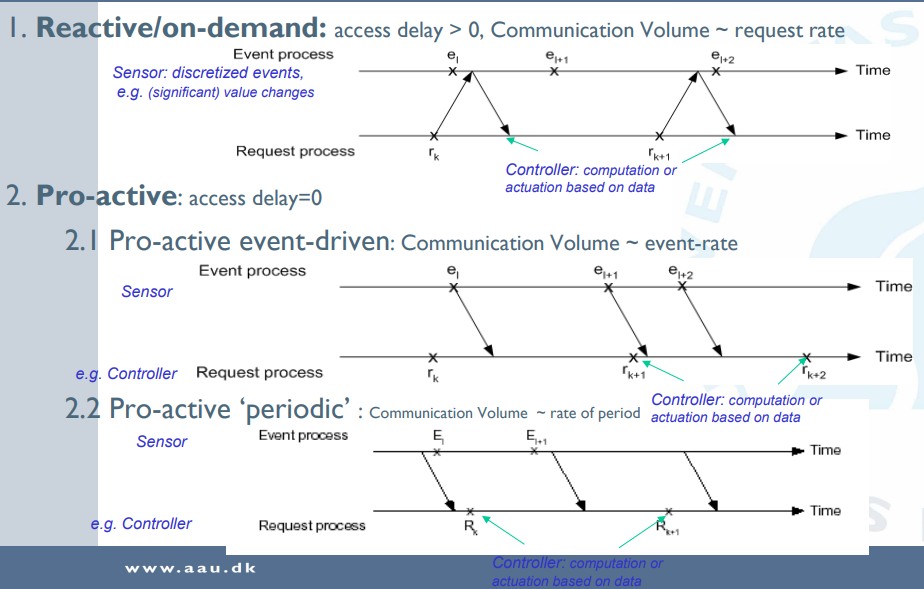
\includegraphics[width=\linewidth]{accessStragies.png}
\end{minipage}\hfill
\begin{minipage}[t]{0.42\textwidth}
\vspace{0pt}
\begin{defbox}
\textbf{Processes:}
\begin{itemize}
  \item $\mathcal{E}$ (rate $\lambda$): event process at sensor
  \item $\mathcal{R}$ (rate $\mu$): request process (reactive only)
  \item $\mathcal{D}$ (rate $\nu$): downstream delay sensor$\to$ctrl
  \item $U$: upstream delay (reactive only)
  \item $\mathcal{P}$ (rate $\tau$): period (proactive periodic only)
\end{itemize}
Together they capture how data moves from sensor to controller.\\[2pt]
\textbf{Assumption:} 
\begin{itemize}
  \item All processes are mutually independent
  \item Message re-ordering can occur in network.
\end{itemize}
\end{defbox}
\end{minipage}

\vspace{4pt}

To compare strategies we need a measure of \textbf{data quality} --- how well does the controller's knowledge match the true sensor value at the moment of computation? For this we use \textbf{mmPr}:

\vspace{2pt}

\begin{keybox}
  Which is the Probability that controller value does not match sensor value, desribed by: \vspace{0.5em}
  \begin{center}
\textbf{mmPr} $:= \Pr\!\left(X_C(C_i) \neq X_s(C_i)\right)$ 
\end{center}
\vspace{0.5em}
\begin{itemize}
  \item $X_s(C_i)$: true sensor value at computation instant $C_i$
  \item $X_C(C_i)$: controller's knowledge of sensor value at $C_i$
\end{itemize}
\textbf{Goal:} minimise mmPr $\approx$ minimise accumulated turbine damage.
\end{keybox}

\vspace{2pt}

% ===========================================================================
\section*{2\quad Analysis: mmPr Formulas}
% ===========================================================================

We analyse mmPr for the 3 access schemes under the assumptions:
\begin{itemize}
  \item Poisson event process at sensor (rate $\lambda$)
  \item General downstream delay $\mathcal{D}$ with distribution $f_D$ (rate $\nu$ for exponential case)
\end{itemize}
Result: two of the three schemes yield the \textbf{same} mmPr --- and the periodic scheme introduces a fundamental floor independent of network speed.

\vspace{1pt}

\begin{minipage}[t]{0.47\textwidth}
\vspace{0pt}
\begin{keybox}
\textbf{Reactive \& Proactive event-driven --- surprisingly same result.}\\[2pt]
Since all processes are independent, $\mathcal{R}$ is \textbf{irrelevant} for stationary mmPr --- both ask the same question:\\[2pt]
\textbf{Reactive:} did a new event occur while waiting for the response?\\[1pt]
\textbf{Proactive (Full updates):} did a new event occur while the last update was in transit?\\[2pt]
Both reduce to: \emph{did the most recent message arrive before the next event?}
\[ \mathrm{mmPr} = 1 - \mathcal{L}\{f_D\}(\lambda) \;\xrightarrow{\text{exp.\ delay}}\; \frac{\lambda}{\lambda+\nu} \]
Large $\nu$: mmPr $\to 0$. \quad Large $\lambda$: mmPr $\to 1$.
\end{keybox}
\end{minipage}\hfill
\begin{minipage}[t]{0.49\textwidth}
\vspace{0pt}
\begin{keybox}
\textbf{Proactive periodic} --- sensor sends at fixed rate $\tau$. More complex than reactive since packets are sent continuously $\Rightarrow$ \textbf{multiple in transit} simultaneously. Model with a \textbf{CTMC} tracking packets in flight.\\[3pt]
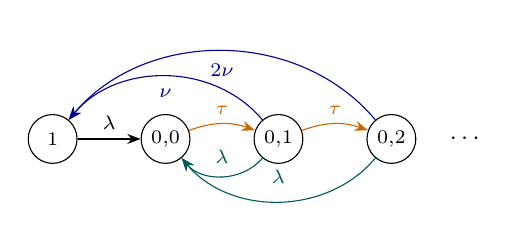
\begin{tikzpicture}[>=Stealth, font=\scriptsize, node distance=0.2cm]
  \node[draw, circle, minimum size=0.62cm, inner sep=0pt] (m) {$1$};
  \node[draw, circle, minimum size=0.62cm, inner sep=0pt, right=0.80cm of m] (a) {$0,\!0$};
  \node[draw, circle, minimum size=0.62cm, inner sep=0pt, right=0.80cm of a] (b) {$0,\!1$};
  \node[draw, circle, minimum size=0.62cm, inner sep=0pt, right=0.80cm of b] (c) {$0,\!2$};
  \node[right=0.30cm of c, font=\small] {$\cdots$};
  % λ: 1→0,0 (straight)
  \draw[->] (m) -- node[above, font=\scriptsize]{$\lambda$} (a);
  % λ: 0,k→0,0 (bent above, teal)
  \draw[->, teal!70!black] (b) to[bend left=50] node[above, font=\scriptsize, yshift=1pt]{$\lambda$} (a);
  \draw[->, teal!70!black] (c) to[bend left=50] node[above, font=\scriptsize, yshift=3pt]{$\lambda$} (a);
  % τ: rightward (orange, bent slightly below to separate from λ)
  \draw[->, orange!80!black] (a) to[bend left=20] node[above, font=\scriptsize]{$\tau$} (b);
  \draw[->, orange!80!black] (b) to[bend left=20] node[above, font=\scriptsize]{$\tau$} (c);
  % ν: service, bent below (blue)
  \draw[->, blue!60!black] (b) to[bend right=50] node[below, font=\scriptsize, yshift=-1pt]{$\nu$} (m);
  \draw[->, blue!60!black] (c) to[bend right=50] node[below, font=\scriptsize, yshift=-1pt]{$2\nu$} (m);
\end{tikzpicture}\\[2pt]
\begin{itemize}
  \item \footnotesize\textbf{1}: matching;
  \item \textbf{0,0}: MM, 0 pkts sent, no in transit but event has happened;
  \item \textbf{0,k}: MM, $k$ in transit.
\end{itemize}
Lowest mmPr $\to \lambda/(\lambda{+}\tau)$ as $\nu\to\infty$. \textbf{$\tau$ always dictates lower bound} --- even if network is infinitely fast.
\end{keybox}
\end{minipage}

\vspace{2pt}

\begin{notebox}
\footnotesize\textbf{Note --- incremental (not used in presentation):} proactive event-driven \emph{incremental updates} = MM $\Leftrightarrow$ $\mathcal{E}/\mathcal{D}/\infty$ queue busy $\Rightarrow$ mmPr $= 1-e^{-\lambda/\nu}$ (Poisson). Delay-distribution-independent.
\end{notebox}

\vspace{2pt}

% ===========================================================================
\section*{3\quad Wind-Farm Timing Model: Offset $T_o$}
% ===========================================================================
Even though proactive periodic has the worst mmPr floor ($\lambda/(\lambda{+}\tau)$) on fast networks, it is used in the wind-farm because the system demands deterministic, scheduled communication. This means we must choose not only the period $T_s = 1/\tau$ but also \textbf{when} within the period to send --- controlled via offset $T_o$.

\vspace{0pt}
\begin{minipage}[t]{0.4\textwidth}
\vspace{0pt}
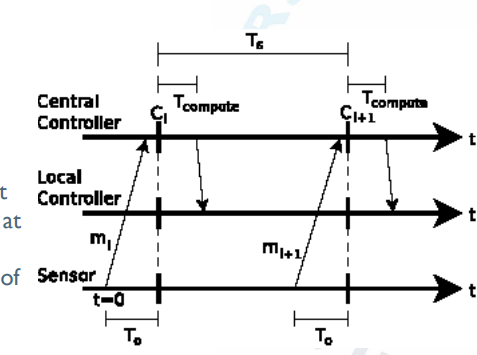
\includegraphics[width=\linewidth]{offsetcomputation.png}
\end{minipage}\hfill
\begin{minipage}[t]{0.51\textwidth}
\vspace{0pt}
\begin{keybox}
$T_s=150\,\text{ms}$, $T_\text{compute}=50\,\text{ms}$, $T_o$=offset (sensor sends $T_o$ before $C_i$).\\[3pt]
\textbf{Trade-off:} 
\begin{itemize}
  \item larger $T_o$ $\Rightarrow$ more time for delivery (fewer misses) but larger info age (data may have changed).
  \item small $T_o$ $\Rightarrow$ less time for delivery (higher miss risk) but fresher data (low info age).
  \item Optimal $T_o\approx100\,\text{ms}$ balances both.
\end{itemize} 
\end{keybox}
\begin{warnbox}
Simulation can find optimal $T_o$ but is \textbf{very expensive}: must run a full control simulation for every candidate $T_o$ value.\\[2pt]
Instead: \textbf{Markov chain data quality model} --- compute mmPr$(\varepsilon)$ analytically as a function of $T_o$, then minimise directly. Much faster; gives same optimal $T_o$.\\[2pt]
Here mmPr$(\varepsilon)$ is the full threshold version:
\[ \mathrm{mmPr}(\varepsilon) := \Pr\!\left(|X_s(C_i) - X_C(C_i)| > \varepsilon\right) \]
$\varepsilon$ is a percentile threshold on the sensor value error
\end{warnbox}
\end{minipage}


% ===========================================================================
\section*{4\quad Data Quality Model: Markov Chain Approaches}
% ===========================================================================

\vspace{0pt}
\begin{minipage}[t]{0.35\textwidth}
\vspace{0pt}
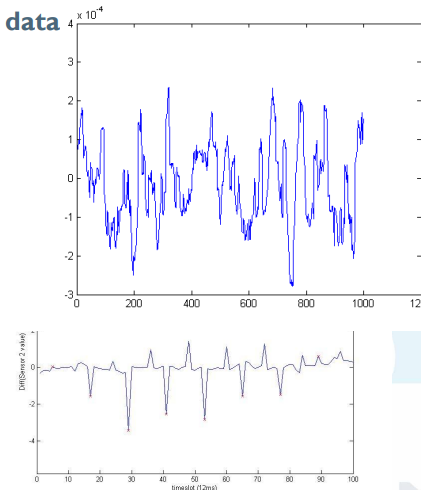
\includegraphics[width=\linewidth]{tworegime.png}
\end{minipage}\hfill
\begin{minipage}[t]{0.55\textwidth}
\vspace{0pt}
\begin{keybox}
\small\textbf{Why Markov?} Sensor data has \textbf{two regimes}:\\[2pt]
\textbf{(1) Normal:} gradual drift between actuations.\\
\textbf{(2) Actuation event:} sudden large jump (downward peaks in diff.\ series).\\[2pt]
$\Rightarrow$ Discretise sensor value space into $N$ states; model transitions as Markov chain.
\end{keybox}
\begin{defbox}
\textbf{Approach I} (empirical):
\begin{itemize}
  \item Run control simulation (e.g.\ ideal scenario)
  \item Take all sensor measurements $\Rightarrow$ snapshot
  \item Discretise into $N$ bins; estimate $N{\times}N$ transition matrix directly from data
  \item Steady-state $\underline{\pi}$ $\Rightarrow$ compute mmPr$(\varepsilon)$
\end{itemize}
Simple, but still requires a full simulation run.
\end{defbox}
\begin{defbox}
\textbf{Approach II} (analytical):
\begin{itemize}
  \item Same $N$-state discretisation
  \item Separate matrices: $P$ (normal transitions) $+$ $C$ (actuation jumps)
  \item $1{-}\mathrm{mmPr}(\varepsilon) = F_D(T_o)\!\sum_k \pi_u(k)\cdot\Pr(k_i\mid k_{i-1})$
  \item Fully analytical as function of $T_o$ $\Rightarrow$ minimise directly
\end{itemize}
\textbf{Heuristic:} $T_o = p$-percentile of delay ($p\approx90\%$).
\end{defbox}
\end{minipage}

\vspace{3pt}

% ===========================================================================
\section*{5\quad Controller Performance \& Data Quality Validation}
% ===========================================================================


\vspace{0pt}
\begin{minipage}[t]{0.31\textwidth}
\vspace{0pt}
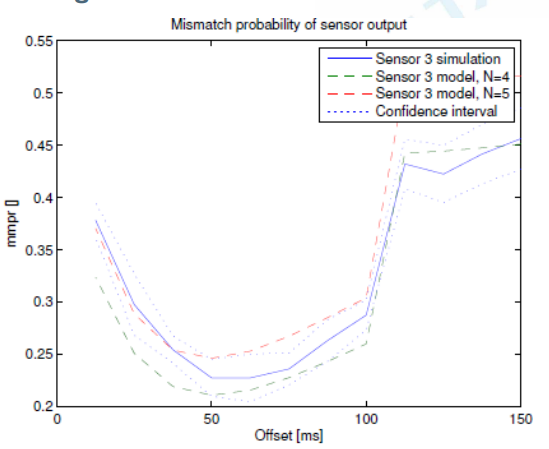
\includegraphics[width=\linewidth]{karmovvssim.png}
\end{minipage}\hfill
\begin{minipage}[t]{0.31\textwidth}
\vspace{0pt}
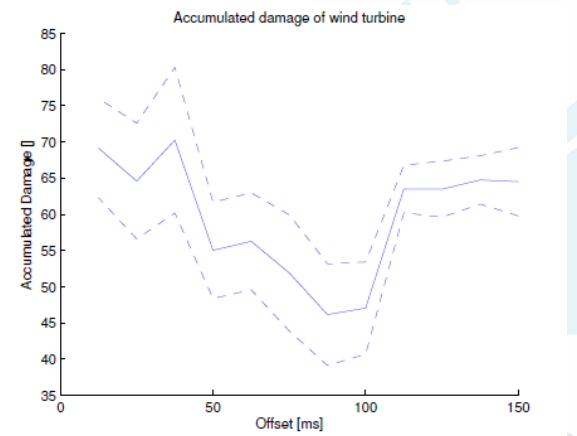
\includegraphics[width=\linewidth]{damageoffset.png}
\end{minipage}\hfill
\begin{minipage}[t]{0.33\textwidth}
\vspace{0pt}
\begin{keybox}
\textbf{Conclusion:} Markov model at $N{=}4$ or $5$ already closely matches simulation --- low $N$ is sufficient.\\[2pt]
\textbf{mmPr $\not\equiv$ min.\ damage exactly} --- damage curve has its minimum at similar $T_o$ but not identical. Use mmPr as a fast analytical \textbf{indicator} to locate optimal $T_o$ without expensive damage simulations.
\end{keybox}
\end{minipage}

\vspace{3pt}


% ===========================================================================
\section*{6\quad Quantitative Results}
% ===========================================================================

\vspace{0pt}
\begin{minipage}[t]{0.45\textwidth}
\vspace{0pt}
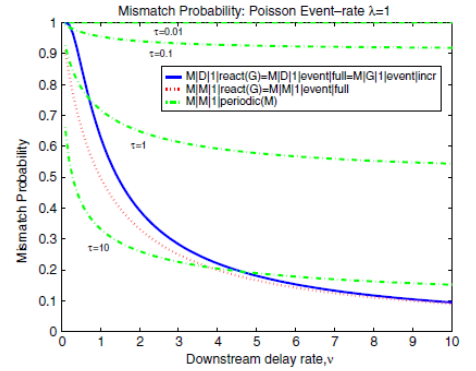
\includegraphics[width=\linewidth]{mmpr.png}
\end{minipage}\hfill
\begin{minipage}[t]{0.44\textwidth}
\vspace{0pt}
\begin{warnbox}
\footnotesize\textbf{Key results ($\lambda=1$):}\\[2pt]
\textbf{Det.\ delay $D$:} reactive $=$ event-driven full $=$ incremental [blue]:
\[ \mathrm{mmPr} = 1 - e^{-\lambda D} \]
Incremental is delay-distribution-independent.\\[2pt]
\textbf{Exp.\ delays} [red]: $\mathrm{mmPr}=\lambda/(\lambda{+}\nu)$ --- \emph{better} than det.\\[2pt]
\textbf{Periodic} [green, $\tau$-labelled]: converges to $\lambda/(\lambda{+}\tau)$ for large $\nu$ --- \emph{worse} because $\tau \ll \nu$.
\end{warnbox}
\end{minipage}


\vspace{3pt}

\end{document}
